% WR figure exported by sim_ui.py -- 2026-09-18 14:44:36
%
% Preamble (once, in your thesis):
%   \usepackage{pgfplots}
%   \pgfplotsset{compat=1.18}
%
% Use:
%   \begin{figure}[htbp]\centering
%     \input{wr_convergence}
%     \caption{...}\label{fig:...}
%   \end{figure}
%
% \input nests (unlike \include), so this works inside a chapter file the root
% already \includes. Pasting the body below inline works too -- the \definecolor
% lines may then be hoisted into the preamble and dropped from each figure.
%
% Series are thinned to ~2000 points each (min/max decimation, so spikes are
% preserved); edit _PGF_MAX_PTS in sim_ui.py for the full-resolution data.
%
% Run: coupling_mode=voltage-driven; precondition=on (optimized); interface_form=Thevenin (V source); use_t_floor=bare dt; interface_consistency=BDF-1/BE (naive); N_field_windows=100; N_xyce_samples=200; xyce_integration_method=Backward-Euler (maxord=1)

\definecolor{C0}{HTML}{1F77B4}
\definecolor{C1}{HTML}{FF7F0E}
\definecolor{C2}{HTML}{2CA02C}
\definecolor{C3}{HTML}{D62728}

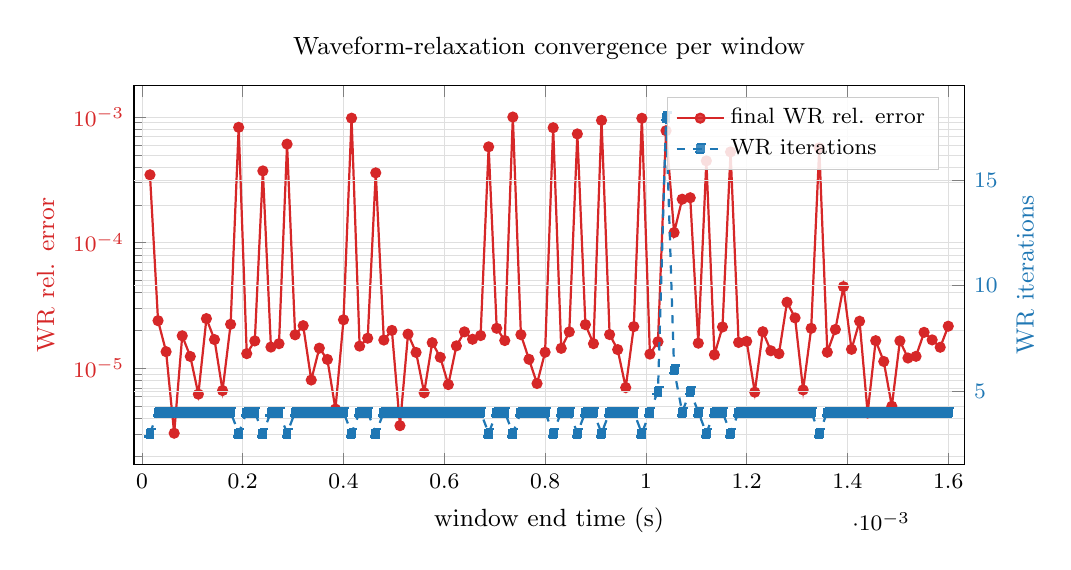
\begin{tikzpicture}
\begin{axis}[
  width=\linewidth,
  height=6.4cm,
  title={Waveform-relaxation convergence per window},
  xlabel={window end time (s)},
  ylabel={WR rel. error},
  grid=both,
  grid style={line width=.2pt, draw=gray!25},
  legend pos=north east,
  legend cell align=left,
  legend style={font=\footnotesize, fill=white, fill opacity=0.85, text opacity=1, draw=gray!40},
  tick label style={font=\footnotesize},
  label style={font=\small},
  title style={font=\small},
  scaled x ticks=true,
  xmin=-1.568e-05,
  xmax=0.00163168,
  ymode=log,
  axis y line*=left,
  ylabel style={color=C3},
  yticklabel style={color=C3}
]
  \addplot[color=C3, line width=0.8pt, mark=*, mark size=1.6pt] coordinates {
    (1.6e-05,0.0003469) (3.2e-05,2.399e-05) (4.8e-05,1.36e-05) (6.4e-05,3.057e-06) (8e-05,1.82e-05) (9.6e-05,1.246e-05)
    (0.000112,6.248e-06) (0.000128,2.493e-05) (0.000144,1.698e-05) (0.00016,6.674e-06) (0.000176,2.246e-05) (0.000192,0.0008272)
    (0.000208,1.312e-05) (0.000224,1.656e-05) (0.00024,0.0003724) (0.000256,1.48e-05) (0.000272,1.574e-05) (0.000288,0.0006083)
    (0.000304,1.853e-05) (0.00032,2.19e-05) (0.000336,8.1e-06) (0.000352,1.451e-05) (0.000368,1.18e-05) (0.000384,4.756e-06)
    (0.0004,2.439e-05) (0.000416,0.0009785) (0.000432,1.506e-05) (0.000448,1.741e-05) (0.000464,0.0003595) (0.00048,1.683e-05)
    (0.000496,2.008e-05) (0.000512,3.509e-06) (0.000528,1.876e-05) (0.000544,1.341e-05) (0.00056,6.415e-06) (0.000576,1.604e-05)
    (0.000592,1.227e-05) (0.000608,7.445e-06) (0.000624,1.513e-05) (0.00064,1.955e-05) (0.000656,1.708e-05) (0.000672,1.827e-05)
    (0.000688,0.0005788) (0.000704,2.087e-05) (0.00072,1.668e-05) (0.000736,0.0009989) (0.000752,1.858e-05) (0.000768,1.183e-05)
    (0.000784,7.594e-06) (0.0008,1.346e-05) (0.000816,0.0008214) (0.000832,1.446e-05) (0.000848,1.955e-05) (0.000864,0.0007335)
    (0.00088,2.231e-05) (0.000896,1.575e-05) (0.000912,0.0009402) (0.000928,1.861e-05) (0.000944,1.413e-05) (0.00096,7.05e-06)
    (0.000976,2.153e-05) (0.000992,0.0009766) (0.001008,1.301e-05) (0.001024,1.632e-05) (0.00104,0.0007773) (0.001056,0.0001205)
    (0.001072,0.0002219) (0.001088,0.0002279) (0.001104,1.589e-05) (0.00112,0.0004478) (0.001136,1.286e-05) (0.001152,2.138e-05)
    (0.001168,0.0005277) (0.001184,1.611e-05) (0.0012,1.644e-05) (0.001216,6.48e-06) (0.001232,1.96e-05) (0.001248,1.383e-05)
    (0.001264,1.311e-05) (0.00128,3.365e-05) (0.001296,2.525e-05) (0.001312,6.753e-06) (0.001328,2.086e-05) (0.001344,0.0005675)
    (0.00136,1.347e-05) (0.001376,2.043e-05) (0.001392,4.473e-05) (0.001408,1.42e-05) (0.001424,2.375e-05) (0.00144,4.428e-06)
    (0.001456,1.664e-05) (0.001472,1.137e-05) (0.001488,5.009e-06) (0.001504,1.658e-05) (0.00152,1.211e-05) (0.001536,1.249e-05)
    (0.001552,1.938e-05) (0.001568,1.688e-05) (0.001584,1.475e-05) (0.0016,2.169e-05)
  };
\end{axis}
\begin{axis}[
  width=\linewidth,
  height=6.4cm,
  title={},
  xlabel={},
  ylabel={WR iterations},
  grid=both,
  grid style={line width=.2pt, draw=gray!25},
  legend pos=north east,
  legend cell align=left,
  legend style={font=\footnotesize, fill=white, fill opacity=0.85, text opacity=1, draw=gray!40},
  tick label style={font=\footnotesize},
  label style={font=\small},
  title style={font=\small},
  scaled x ticks=true,
  xmin=-1.568e-05,
  xmax=0.00163168,
  axis y line*=right,
  axis x line=none,
  ylabel style={color=C0},
  yticklabel style={color=C0}
]
  \addlegendimage{color=C3, line width=0.8pt, mark=*, mark size=1.6pt}
  \addlegendentry{final WR rel. error}
  \addplot[color=C0, line width=0.8pt, dashed, mark=square*, mark size=1.6pt] coordinates {
    (1.6e-05,3) (3.2e-05,4) (4.8e-05,4) (6.4e-05,4) (8e-05,4) (9.6e-05,4)
    (0.000112,4) (0.000128,4) (0.000144,4) (0.00016,4) (0.000176,4) (0.000192,3)
    (0.000208,4) (0.000224,4) (0.00024,3) (0.000256,4) (0.000272,4) (0.000288,3)
    (0.000304,4) (0.00032,4) (0.000336,4) (0.000352,4) (0.000368,4) (0.000384,4)
    (0.0004,4) (0.000416,3) (0.000432,4) (0.000448,4) (0.000464,3) (0.00048,4)
    (0.000496,4) (0.000512,4) (0.000528,4) (0.000544,4) (0.00056,4) (0.000576,4)
    (0.000592,4) (0.000608,4) (0.000624,4) (0.00064,4) (0.000656,4) (0.000672,4)
    (0.000688,3) (0.000704,4) (0.00072,4) (0.000736,3) (0.000752,4) (0.000768,4)
    (0.000784,4) (0.0008,4) (0.000816,3) (0.000832,4) (0.000848,4) (0.000864,3)
    (0.00088,4) (0.000896,4) (0.000912,3) (0.000928,4) (0.000944,4) (0.00096,4)
    (0.000976,4) (0.000992,3) (0.001008,4) (0.001024,5) (0.00104,18) (0.001056,6)
    (0.001072,4) (0.001088,5) (0.001104,4) (0.00112,3) (0.001136,4) (0.001152,4)
    (0.001168,3) (0.001184,4) (0.0012,4) (0.001216,4) (0.001232,4) (0.001248,4)
    (0.001264,4) (0.00128,4) (0.001296,4) (0.001312,4) (0.001328,4) (0.001344,3)
    (0.00136,4) (0.001376,4) (0.001392,4) (0.001408,4) (0.001424,4) (0.00144,4)
    (0.001456,4) (0.001472,4) (0.001488,4) (0.001504,4) (0.00152,4) (0.001536,4)
    (0.001552,4) (0.001568,4) (0.001584,4) (0.0016,4)
  };
  \addlegendentry{WR iterations}
\end{axis}
\end{tikzpicture}
